\documentclass{article}

% Document extensibility %
%
% Disables native paragraph indentation
\usepackage{parskip} 
%
% Provides further bullet options for lists
\usepackage{enumitem}

% Mathematical symbol and statement packages %
%
% Necessary
\usepackage{amsmath}
\usepackage{amssymb}
%
% Extensive fraction notation
\usepackage{xfrac}
%
% Generic mathematical commands
% Notable: \degree, \celcius
\usepackage{gensymb}
%
% Variable vector notation (arrow above variable)
\usepackage{esvect}
%
% Multiline boxed equations
\usepackage{empheq}
%
% SI Unit
\usepackage{siunitx}
\DeclareSIUnit\mile{mi}
%
% More intuitive arrays/matrices
\usepackage{array}

% Graphic packages %
%
% Diagrams and illustrations
\usepackage{tikz}
%
% Image insertion
\usepackage{graphicx}
\graphicspath{ {./} }

% Document content %
%
% Change title of table of contents
% \renewcommand{\contentsname}{Title}

\begin{document}

% Command `\hr` to insert horizontal rules
\newcommand{\hr}{\par\noindent\rule{\textwidth}{0.4pt}}

% Command to box and center math equations
\newcommand{\bc}[1]{
	\begin{equation*}
		\begin{boxed}
			{#1}
		\end{boxed}
	\end{equation*}
}

% Command for single line equations with a condition
\newcommand{\cond}[2]{
	\ifmmode
		{#1} \quad {#2}
	\else
		$$ {#1} \quad {#2} $$
	\fi
}

\tableofcontents

\section{Inertial Frames of Reference}

\textbf{Reference frame} - framework for measurement:
\begin{itemize}
	\item origin
	\item positive axes
	\item t = 0
\end{itemize}

\subsection{Principle of Relativity}
There is no preferred reference frame. \underline{All} physics is equivalent in \underline{every} frame.

\begin{itemize}
	\item Inertial: Two frames related by only a velocity transformation
	\item Non inertial frames - You can still transform from 1 frame to another, but it requires "fictitious force"
\end{itemize}

In order to notate the relative velocity between two objects,
$$ \vec{v}_\frac{\text{object}}{\text{frame}} $$
Velocity of object with respect to frame

\subsection{Example - Utilizing Relativity/Reference Frames}
\begin{align*}
	\left\| \vec{v}_\frac{W}{E} \right\| & = \SI{0.3}{\meter \per \second} \\
	\left\| \vec{v}_\frac{S}{E} \right\| & = \SI{0.4}{\meter \per \second} \\
	\left\| \vec{v}_\frac{S}{W} \right\| & = ? \\
	\theta & = ?
\end{align*}
Establish vector form
\begin{align*}
	\vec{v}_\frac{S}{E} & = 0 \hat{x} + v_\frac{S}{E}\hat{y} \\
	\vec{v}_\frac{W}{E} & = -v_\frac{W}{E}\hat{x} + 0\hat{y} \\
	\vec{v}_\frac{S}{W} & = v_\frac{S}{W}\sin(\theta)\hat{x} + v_\frac{S}{W}\cos(\theta)\hat{y}
\end{align*}
\begin{align*}
	\vec{v}_\frac{W}{E} + \vec{v}_\frac{S}{W} & = \vec{v}_\frac{S}{E}
\end{align*}
Solving $ x $ components
\begin{align*}
	\vec{v}_{\frac{W}{E}_x} + \vec{v}_{\frac{S}{W}_x} & = \vec{v}_{\frac{S}{E}_x} \\
	-\vec{v}_\frac{W}{E} + \vec{v}_\frac{S}{W}\sin(\theta) & = 0 \\
	\vec{v}_\frac{S}{W}\sin(\theta) & = \vec{v}_\frac{W}{E}
\end{align*}
Solving $ y $ components
\begin{align*}
	\vec{v}_{\frac{W}{E}_y} + \vec{v}_{\frac{S}{W}_y} & = \vec{v}_{\frac{S}{E}_y} \\
	0 + \vec{v}_\frac{S}{W}\cos(\theta) & = \vec{v}_\frac{S}{E} \\
	\vec{v}_\frac{S}{W}\cos(\theta) & = \vec{v}_\frac{S}{E}
\end{align*}
\begin{align*}
	\tan(\theta) & = \frac{\vec{v}_\frac{W}{E}}{\vec{v}_\frac{S}{E}} \\
	\theta & = \arctan \left( \frac{\vec{v}_\frac{W}{E}}{\vec{v}_\frac{S}{E}} \right) \\
	\theta & = \arctan \left( \frac{\vec{v}_\frac{W}{E}}{\vec{v}_\frac{S}{E}} \right) \\
	\theta & = \arctan \left( \frac{\SI{0.3}{\meter \per \second}}{\SI{0.4}{\meter \per \second}} \right) \\
	\theta & = \SI{37}{\degree}
\end{align*}
\begin{align*}
	\vec{v}_\frac{S}{W}\sin(\theta) & = \vec{v}_\frac{W}{E} \\
	\vec{v}_\frac{S}{W} & = \frac{v_\frac{W}{E}}{\sin(\theta)} \\
						& = \frac{\SI{0.3}{\meter \per \second}}{\sin(\SI{37}{\degree})} \\
	\vec{v}_\frac{S}{W} & = \SI{0.5}{\meter \per \second}
\end{align*}

\subsection{Example - Airplane}
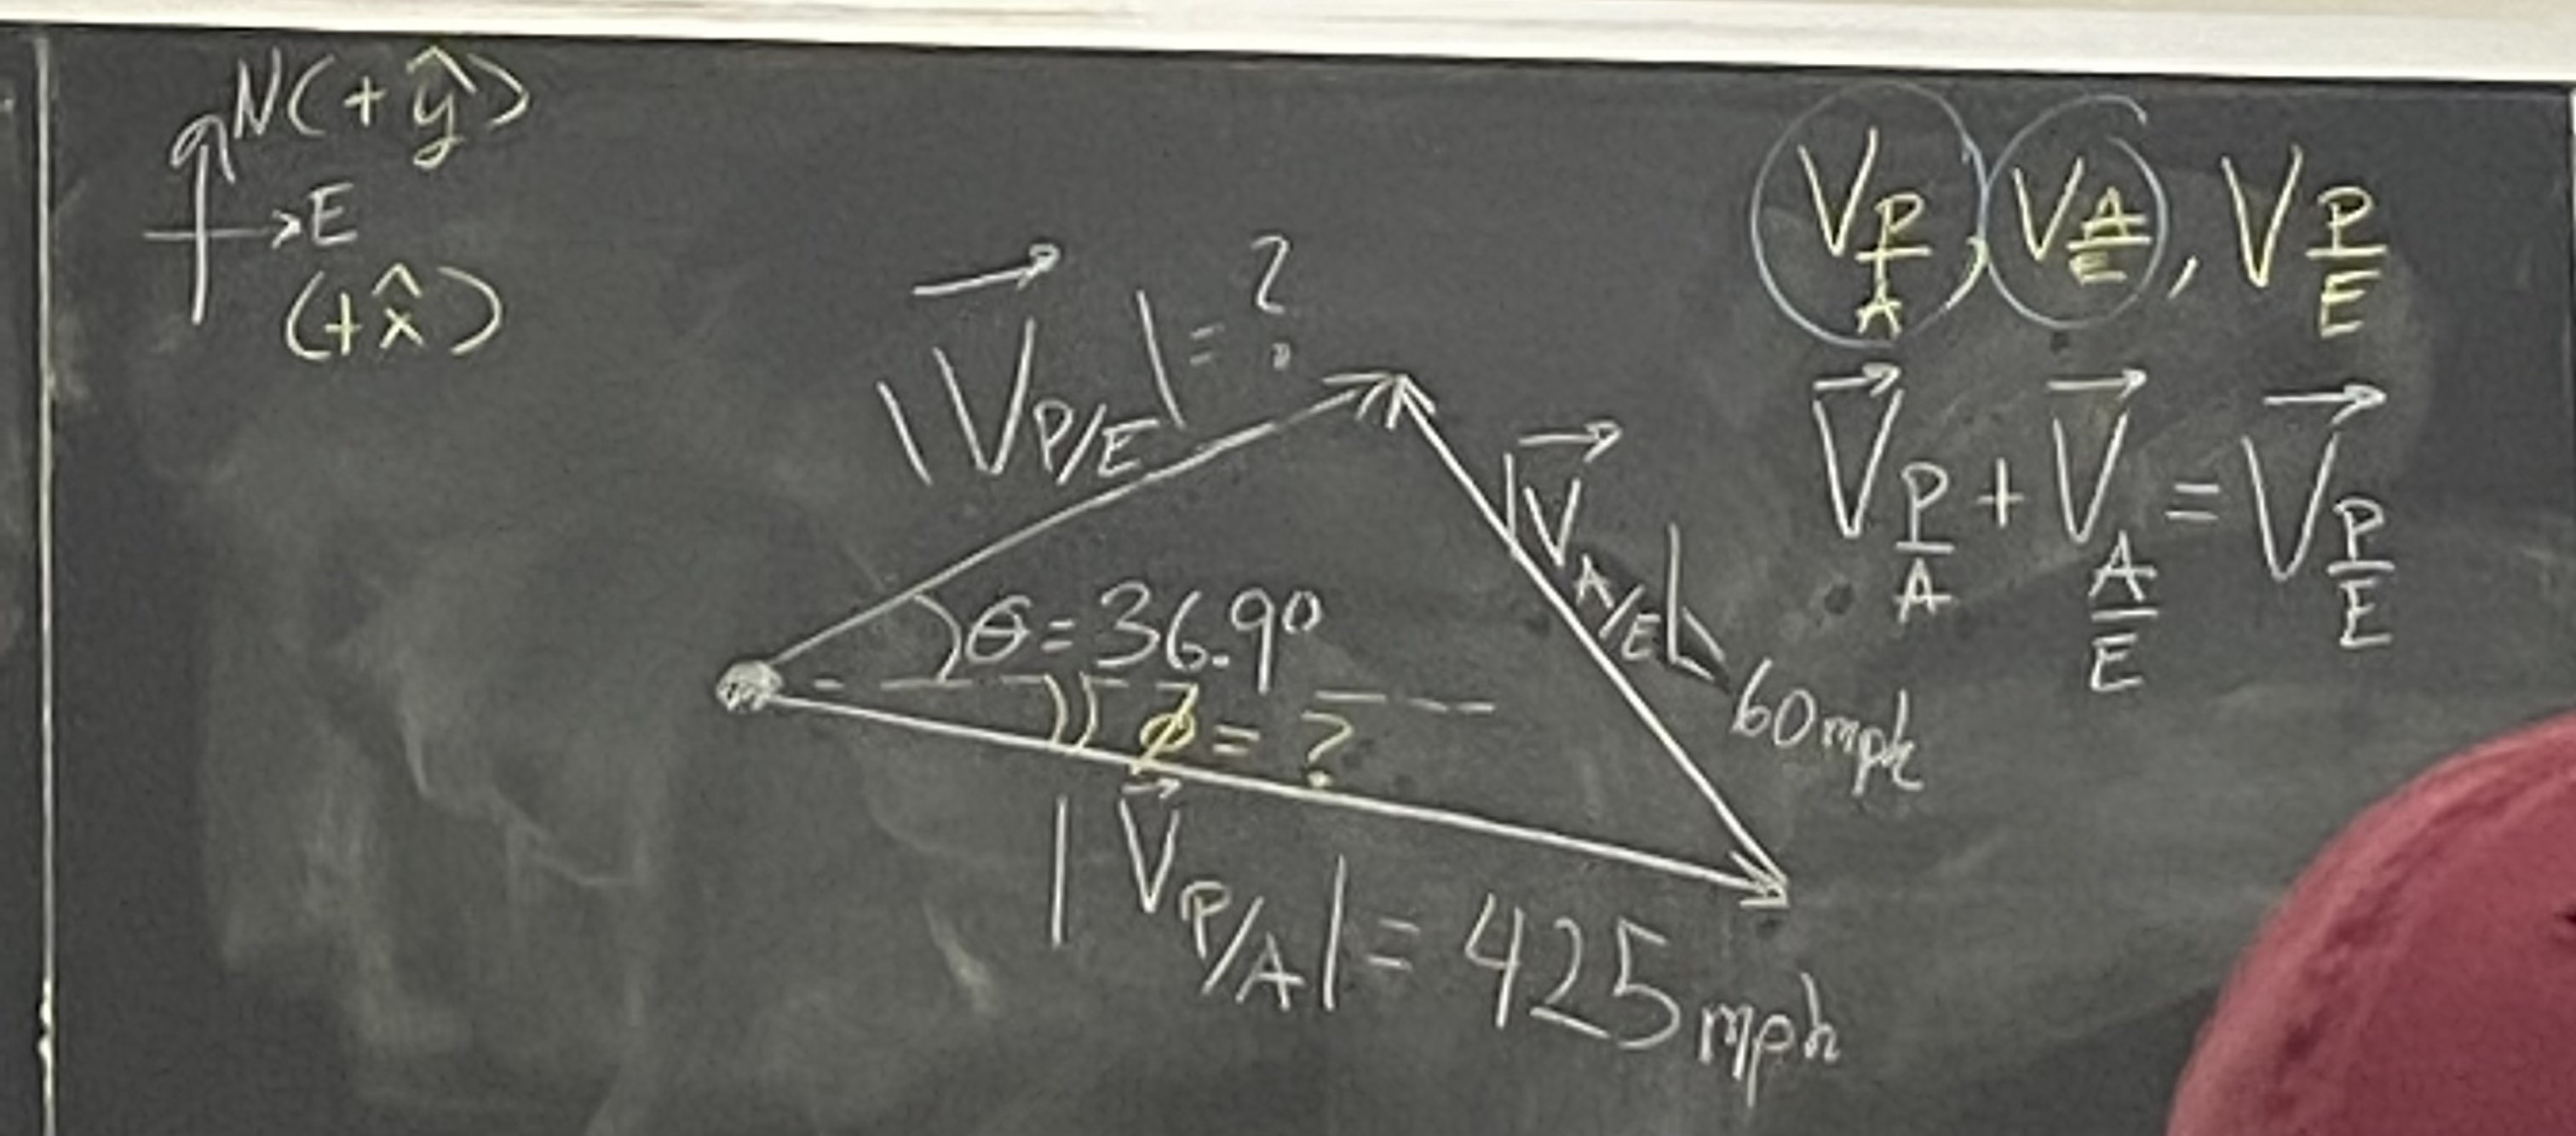
\includegraphics[width=\linewidth]{airplane_graph.jpg}
\begin{align*}
	\theta & = \SI{36.9}{\degree} \\
	\beta & = \SI{45.0}{\degree}
\end{align*}
\begin{align*}
	\vec{v}_\frac{P}{A} & = v_\frac{P}{A}\cos(\phi)\hat{x} - v_\frac{P}{A}\sin(\phi)\hat{y} \\
	\vec{v}_\frac{A}{E} & = -v_\frac{A}{E}\sin(\beta)\hat{x} + v_\frac{A}{E}\cos(\beta)\hat{y} \\
	\vec{v}_\frac{P}{E} & = v_\frac{P}{E}\cos(\theta)\hat{x} + v_\frac{P}{E}\sin(\theta)\hat{y}
\end{align*}
\begin{align*}
	v_{\frac{P}{A}_x} + v_{\frac{P}{E}_x} & = v_{\frac{A}{E}_x} \\
	v_{\frac{P}{A}}\cos(\phi) + v_{\frac{P}{E}}\cos(\theta) & = v_{\frac{A}{E}}\sin(\beta) \\
	(\SI{425}{\mile \per \hour})\cos(\phi) + v_\frac{P}{E}\cos(\SI{36.9}{\degree}) & = (\SI{60}{\mile \per \hour})\sin(\SI{45.0}{\degree})
\end{align*}
\begin{align*}
	v_{\frac{A}{E}_y} + v_{\frac{P}{E}_y} & = v_{\frac{P}{A}_y} \\
	v_{\frac{A}{E}}\cos(\beta) + v_{\frac{P}{E}}\sin(\theta) & = v_{\frac{P}{A}}\sin(\phi) \\
	(\SI{60}{\mile \per \hour})\cos(\SI{45}{\degree}) + v_\frac{P}{E}\sin(\SI{36.9}{\degree}) & = (\SI{425}{\mile \per \hour})\sin(\phi)
\end{align*}

\subsection{Example - Airplane 2}
A pilot wishes to fly due North. Their plane has an airspeed of \SI{300}{\mile \per \hour}. There is a \SI{50}{\mile \per \hour} wind blowing $ \phi = \SI{25}{\degree} $ W of N. What angle $ \theta $, should the pilot steer?
\begin{align*}
	\vec{v}_\frac{P}{E} & = 0\hat{x} + v_\frac{P}{E}\hat{y} \\
	\vec{v}_\frac{A}{E} & = (-\SI{50}{\mile \per \hour})\sin(\SI{25}{\degree})\hat{x} + (\SI{50}{\mile \per \hour})\cos(\SI{25}{\degree}) \\
	\vec{v}_\frac{P}{A} & = (\SI{300}{\mile \per \hour})\cos(\theta)\hat{x} + (\SI{300}{\mile \per \hour})\sin(\theta)\hat{x}
\end{align*}
\begin{align*}
	\vec{v}_{\frac{A}{E}_x} + \vec{v}_{\frac{P}{A}_x} & = \vec{v}_{\frac{P}{E}_x} \\
	(-\SI{50}{\mile \per \hour})\sin(\SI{25}{\degree}) + (\SI{300}{\mile \per \hour})\cos(\theta) & = 0 \\
	\theta & = \arccos \left( \frac{ (\SI{50}{\mile \per \hour})\sin(\SI{25}{\degree}) }{ \SI{300}{\mile \per \hour} } \right) \\
	\theta & = \SI{86.0}{\degree}
\end{align*}

\section{Newton's Second Law}

\begin{align}
	F & \equiv \frac{d\vec{p}}{dt}, \quad \frac{\text{momentum}}{\text{time}} \\
	  & \equiv \frac{dm}{dt}v + m\frac{d\vec{v}}{dt}, \quad \frac{dm}{dt} = 0
\end{align}
\begin{align}
	\sum \vec{F}^{(m)} & = m\vec{a}
\end{align}

\subsection{Example - Pulley}
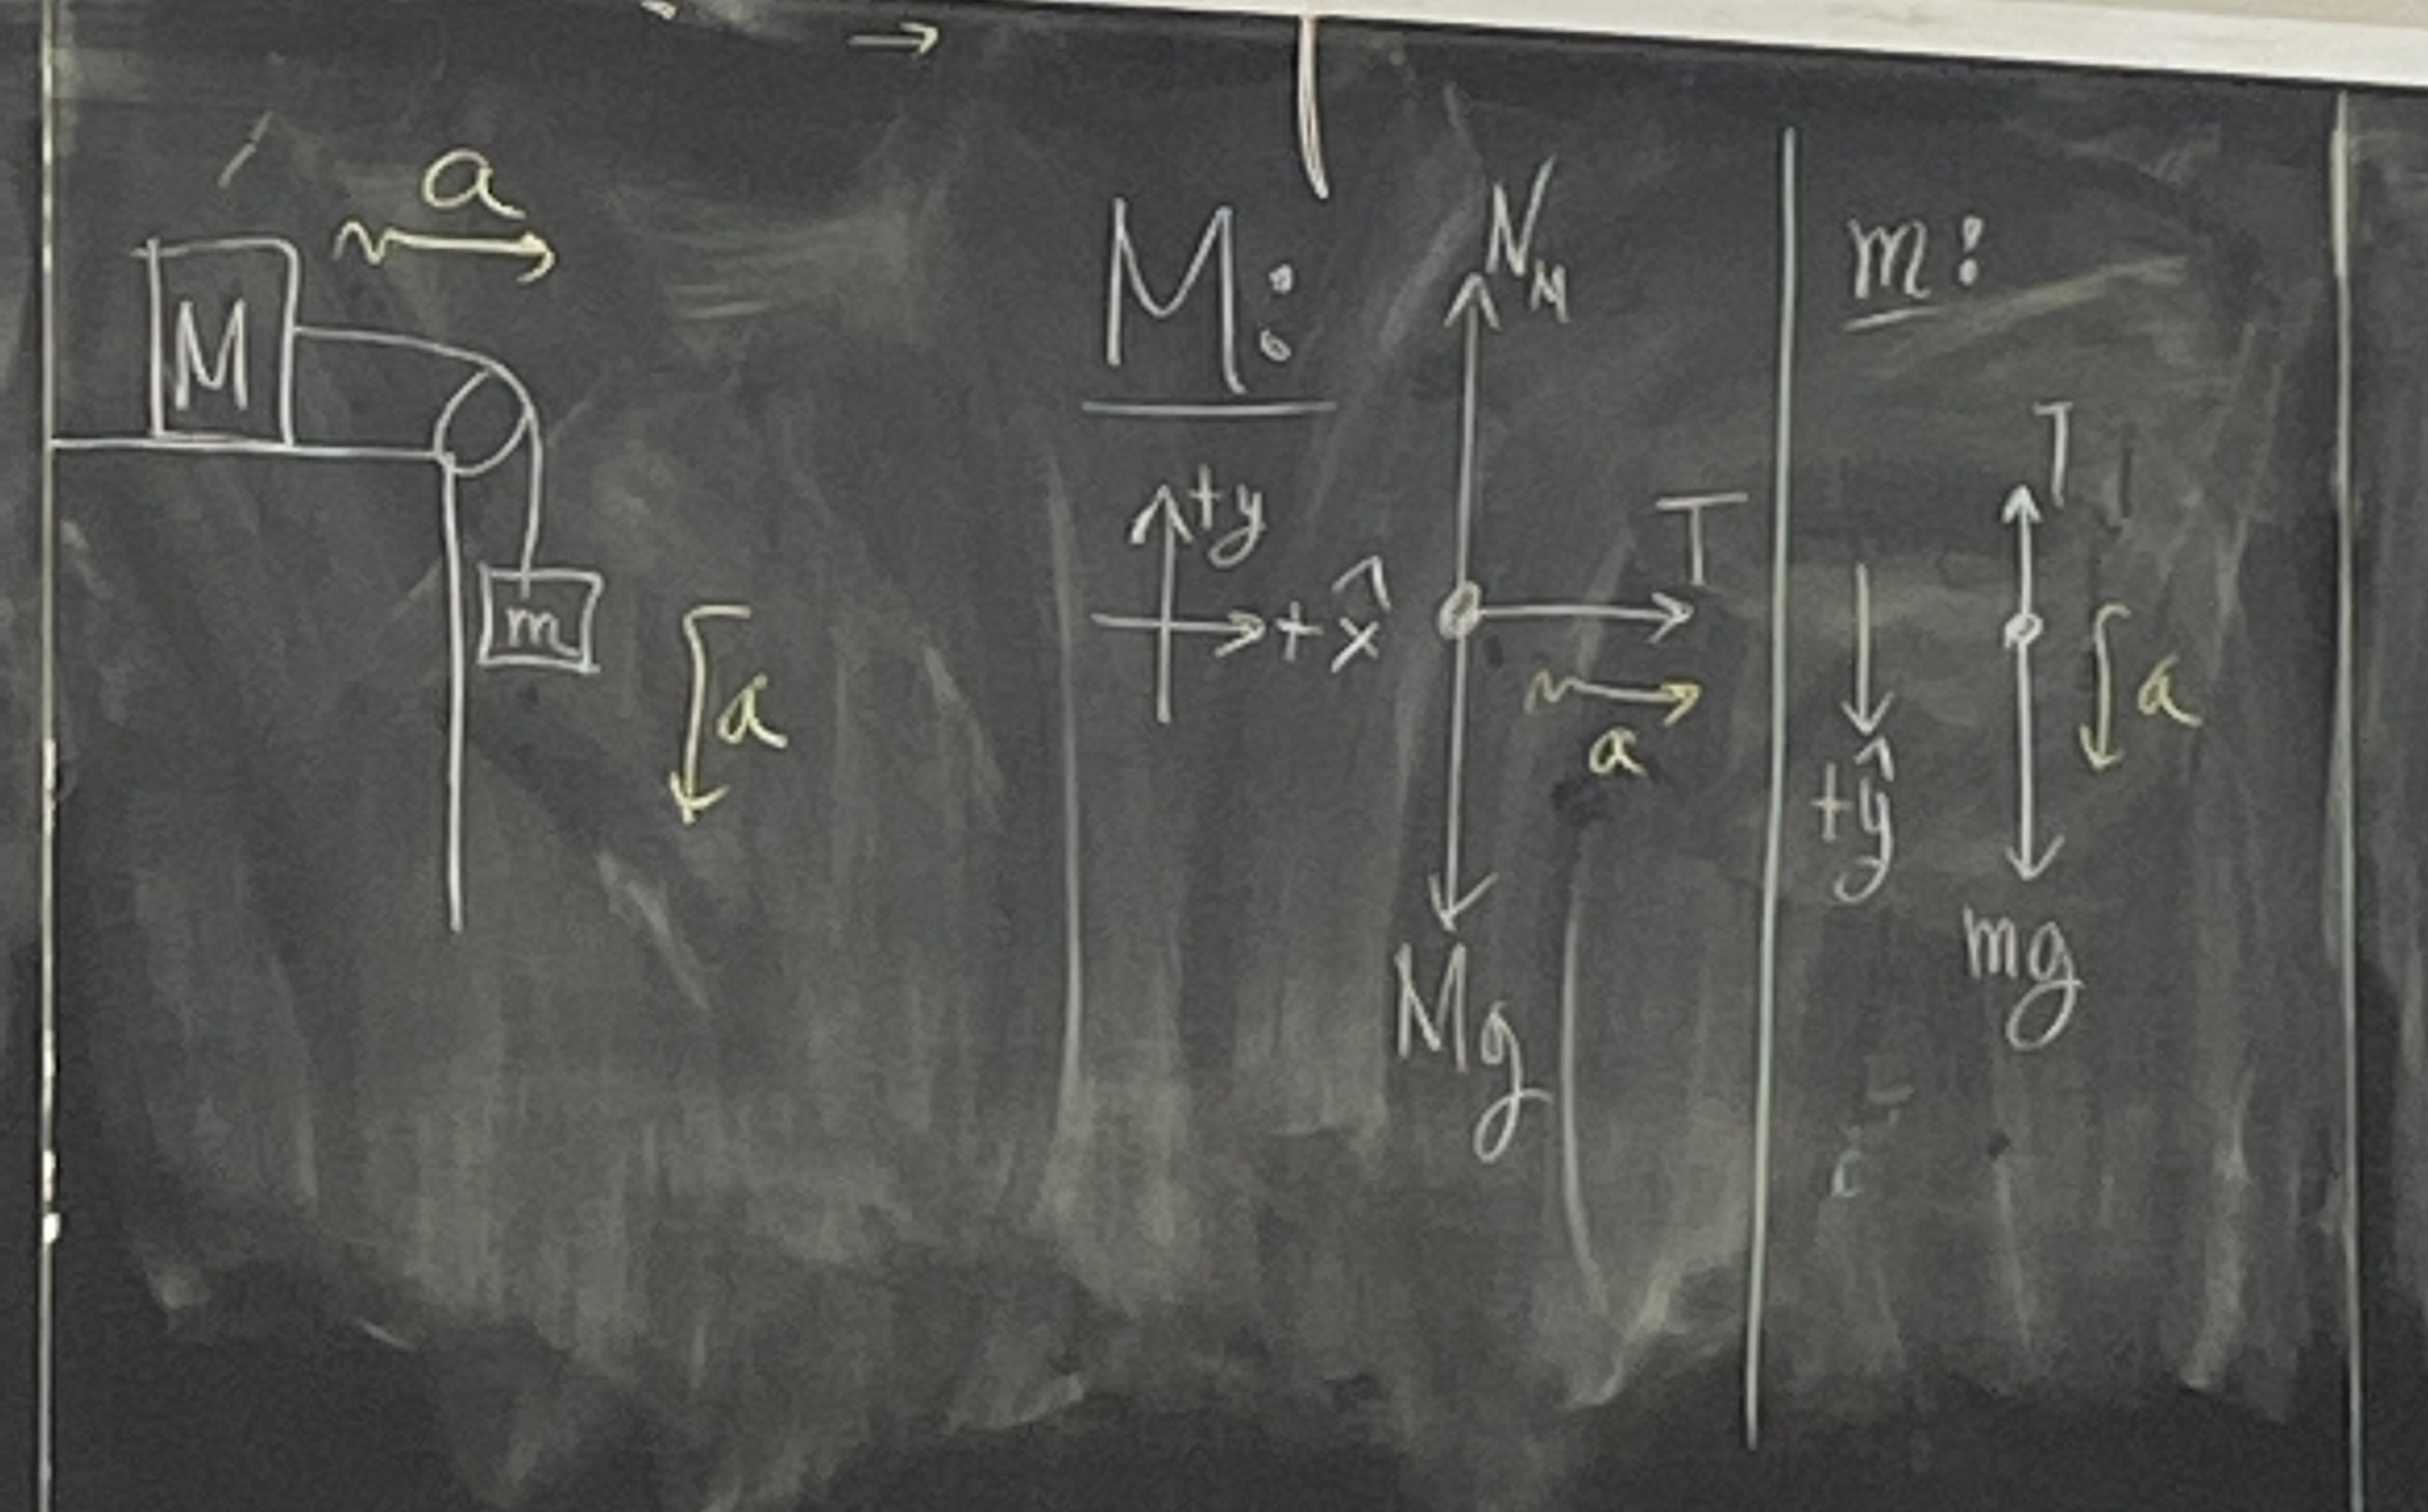
\includegraphics[width=\linewidth]{nsl_pulley.jpg}
Find $ a $ and $ T $
\begin{align*}
	\sum F_{x}^{(M)} & = Ma \\
	T & = Ma
\end{align*}
\begin{align*}
	\sum F_{y}^{(M)} & = 0 \\
	N_M & = Mg
\end{align*}
\begin{align*}
	\sum F_y^{(m)} & = ma \\
	mg - T & = ma \\
	mg - Ma & = ma \\
	a(m + M) & = mg \\
	a & = \frac{mg}{m + M}
\end{align*}
\bc{T = Ma, a = \frac{mg}{m + M}}

\end{document}
